 \documentclass{article}

% preambulo:
\input{Control_tp3_preamble.tex}

\usepackage{fancyhdr}

\geometry{top=2.5cm, bottom=2.0cm, left=2.25cm, right=2.25cm}

\lhead{Sistemas de Control 22.85}
\chead{TP3 - Control Servo}
\rhead{ITBA}
\renewcommand{\headrulewidth}{1pt}
\renewcommand{\footrulewidth}{1pt}
\pagestyle{fancy}


\begin{document}

%\newgeometry{} % margenes default para la caratula
% caratula:
\input{Control_tp3_caratula.tex}


% indice:
\tableofcontents
\newpage

\section{Análisis del Motor de CC}

En primer lugar se considera el modelo circuital para el motor utilizado, teniendo en cuenta que los diferentes parámetros son datos provistos por la hoja de datos del QUANSER:

\begin{figure}[H]
\centering
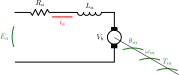
\includegraphics[width=0.5\linewidth]{../Images/ModeloMotor.png}
\end{figure}

Las ecuaciones que caracterizan al sistema son:

\[
\left\lbrace
\begin{array}{ll}
E_a = R_a \cdot i_a + L_a \cdot \dot{i_a} + V_b \\
V_b = K_b \cdot \omega_m = K_b \cdot \dot{\theta_m} \\
T_m = J_m \cdot \ddot{\theta_m} + B_m \cdot \dot{\theta_m} \\
T_m = K_t \cdot i_a
\end{array}
\right.
\]

De las cuales se puede obtener las funciones de transferencia de $\theta_m$ y $\omega_m$ respecto a la tensión de alimentación $E_a$. Considerando que $B_m = 0$, resulta:

\[
\frac{\omega_m}{E_a} = \frac{\frac{K_t}{L_a \cdot J_m}}{S^2 + S\cdot \frac{R_a}{L_a} + \frac{K_t \cdot K_b}{L_a \cdot J_m}}
\]

\[
\frac{\theta_m}{E_a} = \frac{\frac{K_t}{L_a \cdot J_m}}{S\cdot \left(S^2 + S \cdot \frac{R_a}{L_a} + \frac{K_t \cdot K_b}{L_a \cdot J_m}\right)}
\]

De donde se puede construir el diagrama en bloques (en general): 

\begin{figure}[H]
\centering
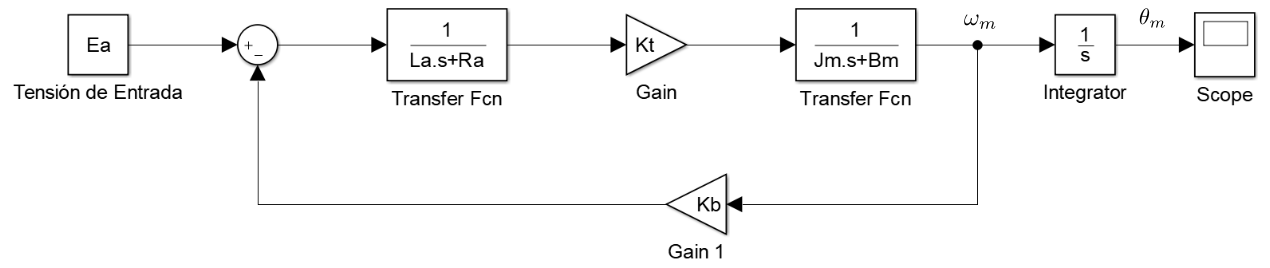
\includegraphics[width=1\linewidth]{../Images/DiagramaSimple.png}
\end{figure}

Donde el valor de las constantes provistas por la hoja de datos son:

\[
R_a = 2.6 [\Omega] \hspace{1cm} J_m = 3.87 \cdot 10^{-7} [Kg \cdot m^2] \hspace{1cm} E_a = 6 [V] \textrm{ (Máximo)} \hspace{1cm} L_a = 180 [\mu Hy] \hspace{1cm}
\]

\[
K_t = 0.00767[Nm] \hspace{1cm} K_b = 0.00767 \left[\frac{V}{rad \cdot seg}\right] 
\]

\[
K_{Pot} = 35.2 \left[ \frac{\circ}{V} \right] \textrm{ (Sobre el potenciómtetro sin las resistencias de }7.15K\Omega)
\]

\[
K_{Tach} = 1.5 \left[  \frac{V}{1000RPM} \right]
\]

\newpage

Al sistema bajo análisis se le aplica realimentación lineal de estados para controlar la posición del motor, tomando como variables de estado a $\omega_m$ y a $\theta_m$. Luego de aplicarla, el diagrama en bloques queda de la forma:

\begin{figure}[H]
\centering
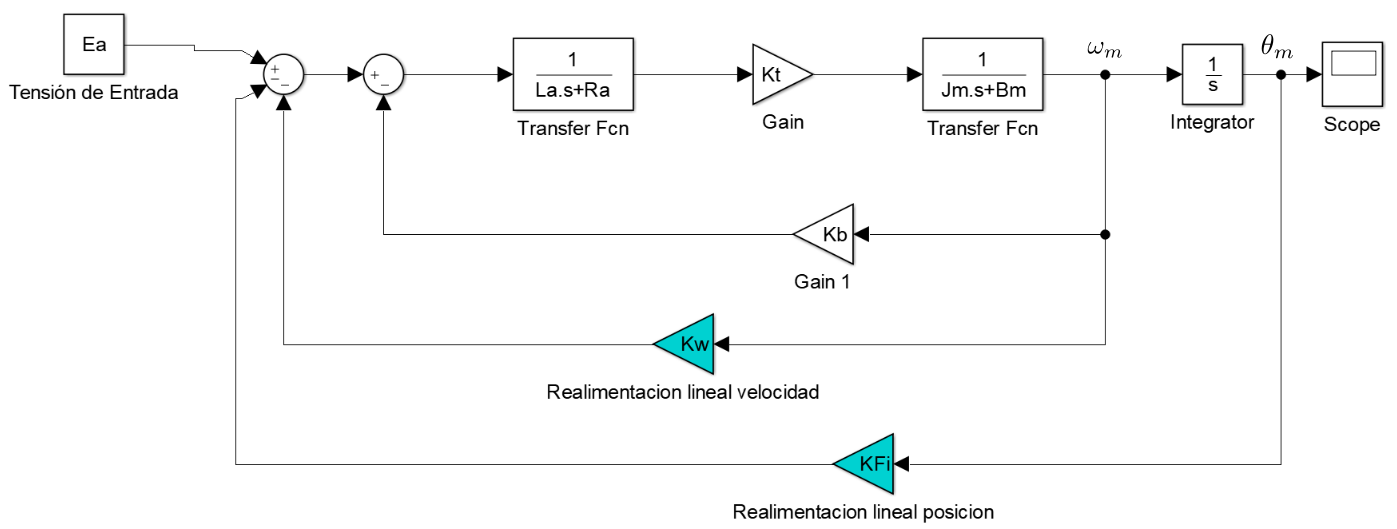
\includegraphics[width=1\linewidth]{../Images/DiagramaFeed.png}
\end{figure}

Para anular el error permanente se agrega delante un bloque de ganancia $K_{Prev}$:

\begin{figure}[H]
\centering
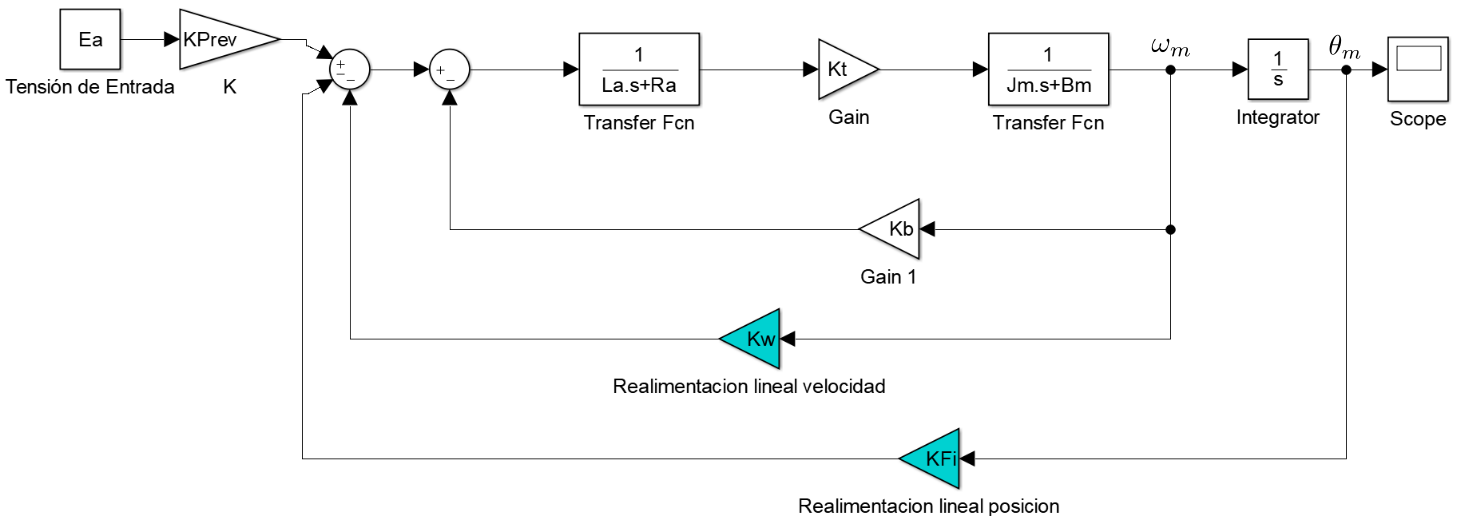
\includegraphics[width=1\linewidth]{../Images/DiagramaFeedConKP.png}
\end{figure}

Para hallar las constantes de realimentación lineal se aplica el método de Ziegler-Nichols en el controlador a implementar, para luego comparar las mediciones que resultan con dichas constantes con la simulación.

\newpage

\section{Controlador Arduino - Código Fuente}
Para realizar la realimentación lineal de estados, se implementó mediante un software en Arduino, cuyo código fuente se cita a continuación.\par
El mapeo del potenciómetro para los extremos de $0^{\circ}$ a $180^{\circ}$ en el ADC (de 10 bits) resulta entre aproximadamente 490 y 740. Pasando estos valores a tensión, resulta:

\[
\frac{490 \cdot 5V}{1023} = 2.4V \hspace{2cm} \frac{740 \cdot 5V}{1023} = 3.6V
\]
Dichos valores equivalentes se utilizarán luego para verificar los extremos de las mediciones frente a entradas de diferentes señales.\par
Se mapean con otras dos entradas de ADC, la señal de entrada $E_a$ y la salida del tacómetro adaptada mediante un driver externo (ver diseño en la siguiente sección). Para simular el nodo sumador, se hace la resta de $E_a$ con las otras dos señales medidas: este resultado corresponde a la señal error, que configura directamente el duty de la señal de control del puente H.

\begin{lstlisting}

#include <L298N.h>
// Libreria para el manejo de la Placa Stepper

#define ADC_MID_RANGE 512 // El rango total es 1024, lo que hace es considerar el offset de la se\~nal a 2.5V
#define PIN_ENABLE 10 // 
#define PIN_IN1 9
#define PIN_IN2 8

#define K_PREV 2.5

#define LIM_SUP 740
#define LIM_INF 490

#define K_TACH 1.5

// Constantes para realimentacion lineal de estados
#define K_FI 1
#define K_W 1

L298N * canalA=NULL;

class polePlacement {       
  private:             
    float kVel;
    float kFi;
    int pinW;
    int pinFi;
    int pinSetPoint;        
    L298N * motor;
 
    configMotorSpeed(int mapedDuty);
   
   public:
   // Inicializador
   polePlacement(int pinEnable, int pinIn1, int pinIn2,int pinW,int pinFi,int pinSetPoint,float kVel,float kFi);
 
   runOnce();
       
};

polePlacement * MotorDrv;

void setup() {
  
  MotorDrv = new polePlacement(PIN_ENABLE,PIN_IN1,PIN_IN2,A0,A1,A2,-4,2.1);

}

void loop() {
 
  MotorDrv->runOnce();
  delay(1); // Muestreo cada 1ms

}

polePlacement::polePlacement(int pinEnable, int pinIn1, int pinIn2,int pinW,int pinFi,int pinSetPoint,float kVel,float kFi){
  this->kVel = kVel;
  this->kFi = kFi;
  this->pinFi = pinFi;
  this->pinW = pinW;
  this->pinSetPoint = pinSetPoint;
  motor = new L298N(pinEnable,pinIn1,pinIn2);
}

polePlacement::runOnce(){

  int medVel, medPos, medSetPoint, e;

  medVel = analogRead(pinW) - ADC_MID_RANGE;
  medPos = analogRead(pinFi);
  medSetPoint = analogRead(pinSetPoint);

  medSetPoint = K_PREV*(medSetPoint-ADC_MID_RANGE);

  medPos = map(medPos, LIM_INF, LIM_SUP, 0, 1023) - ADC_MID_RANGE;
  
  e = medSetPoint-(medPos*kFi)-(medVel*kVel);

  configMotorSpeed(map(e, -512*K_TACH, 512*K_TACH, -255, 255));
  
}

polePlacement::configMotorSpeed(int mapedDuty){
  
  if(mapedDuty > 255){
    mapedDuty = 255;
  }else if(mapedDuty < -255){
    mapedDuty = -255;
  }

  if(mapedDuty < 0){
    motor->setSpeed(-mapedDuty);
    motor->forward();   
  }else{
    motor->setSpeed(mapedDuty);
    motor->backward();    
  }
}

\end{lstlisting}

\newpage

\section{Driver para señales}
Dado que la implementación del controlador se realizó en Arduino, se debieron adaptar las señales de los sensores acorde a los niveles de tensión que admite el Arduino, para lo cual se realizó una placa adicional como driver.

\subsection{Motor - Puente H}
El motor acepta como máxima tensión de alimentación 6V, por lo que alimentando a la placa con $\pm 10$V, se toman los +10V y se pasan por un regulador LM7806, y de ahí se toma la alimentación para el puente H (para el control del motor):

\begin{figure}[H]
\centering
\includegraphics[width=0.4\linewidth]{../Images/Regulador.png}
\end{figure}

Se utilizó la Placa Stepper para Arduino (AR-L298SHIELD), para lo cual se utilizó la librería L298.h mencionada en el código fuente.

\subsection{Potenciómetro (Posición)}

Para el potenciómetro que permite medir la posición angular del motor, se lo alimenta con 6V y se conecta la salida a una de las entradas analógicas de Arduino (A1) en forma directa:

\begin{figure}[H]
\centering
\includegraphics[width=0.15\linewidth]{../Images/PoteMotor.png}
\end{figure}

\subsection{Tacómetro (Velocidad)}
Para adaptar la señal del tacómetro, dado que provee valores entre -5V y +5V, se implementó con un amplificador operacional una función lineal, tal que la salida se mapee al intervalo de 0V a 5V (que es el rango admitido por el Arduino), alimentándolo entre $\pm 10V$: \par

\begin{figure}[H]
\centering
\includegraphics[width=0.4\linewidth]{../Images/ModeloFuncion.png}
\end{figure}

Considerando la transferencia de un amplificador inversor:

\[
A_V = - \frac{R_f}{R_r}
\]

El rango total inicial es de 20V, y el buscado es de 5V, por lo que el factor de escala es 4. De esta forma se toma $R_f = 1K$ y $R_r = 3K9 + 100$ (desdoblando esta última en dos resistencias en serie). Para el offset, se considera el divisor resistivo y la ganancia de un amplificador no inversor, tal que:

\[
10V \cdot \frac{R_B}{R_A + R_B} \cdot \left(1 + \frac{1}{4}\right) = 2.5V
\]

De esta forma el divisor resistivo resulta de $\frac{1}{5}$, por lo que se toma $R_B = 1K$ y $R_A = 3K9 + 100$ (desdoblando esta última en dos resistencias en serie). Finalmente, el circuito resultante es el siguiente:

\begin{figure}[H]
\centering
\includegraphics[width=0.6\linewidth]{../Images/FuncionOpamp.png}
\end{figure}

\subsection{Señal de control por Potenciómetro}

Para el potenciómetro de señal de control manual, utilizando la misma alimentación de 6V saliente del regulador, se le colocó una resistencia en serie tal que la máxima salida sea de 5V:

\begin{figure}[H]
\centering
\includegraphics[width=0.1\linewidth]{../Images/PoteManual.png}
\end{figure}

\subsection{Driver PCB}
Se muestra a continuacón el layout del diseño final de la placa.

\begin{figure}[H]
\centering
\includegraphics[width=0.35\linewidth]{../Images/Top.png}
\centering
\includegraphics[width=0.35\linewidth]{../Images/Bottom.png}
\caption{Diseño de Driver - Lado Top y Bottom}
\end{figure}


\section{Simulación y Mediciones}

Se realizaron ensayos para diferentes tipos de entrada al sistema, considerando señales cuadrada, triangular y senoidal, además de control manual mediante potenciómetro.

\subsection{Entrada por potenciómetro}

En este caso se utilizó el control dado por el potenciómetro configurado según la sección 3.4. El rango de control que permite es de $0^{\circ}$ a $180^{\circ}$. Con esta señal de prueba y con la cuadrada se pudo calibrar la constante de corrección de error permanente $K_{Prev}$ en el software.

\subsection{Entrada por señal}

\subsubsection{Rectangular}
Se ingresa al controlador de Arduino con una señal cuadrada de entre 0V y 5V (y con el software para controlar el puente H se mapea a una señal de entre 0V y 6V). Ajustando las constantes de realimentación lineal de estados en forma experimental tomando de guía el método de Ziegler-Nichols, se logró llegar a un régimen lo más cercano posible al crítico. Se muestran los resultados comparados de la simulación y la medición.

\begin{figure}[H]
\centering
\includegraphics[width=0.6\linewidth]{../Images/EscalonSimulado.png}
\caption{Respuesta al escalón simulada}
\end{figure}

\begin{figure}[H]
\centering
\includegraphics[width=0.45\linewidth]{../Mediciones/servo_cuadrada.jpeg}
\includegraphics[width=0.45\linewidth]{../Images/EscalonMedido.png}
\caption{Respuesta al escalón medida - Detalle de la medición (mediante exportación de CSV)}
\end{figure}

Para comparar correctamente ambos casos, se debe tener en cuenta que la simulación se ingresa con escalón de 6V que es el máximo admitido. En la medición se ingresa con la señal de entrada de máximo 5V para realizar el control a través del Arduino. Se tiene en este caso que el máximo se da a 3.76V (contra los 3.6V teóricos calculados previamente) y mínimo a 2.64V (contra los 2.4V teóricos). En el caso simulado el tiempo de establecimiento resulta de aproximadamente 125ms, mientras que en el medido es de 100ms aproximadamente. Se trabajó con una frecuencia de 0.2Hz.

\newpage

\subsubsection{Triangular}

Se ingresa ahora al controlador de Arduino con una señal triangular de entre 0V y 5V.

\begin{figure}[H]
\centering
\includegraphics[width=0.7\linewidth]{../Images/RampaSimulado.png}
\caption{Respuesta a la rampa simulada}
\end{figure}

\begin{figure}[H]
\centering
\includegraphics[width=0.45\linewidth]{../Mediciones/servo_triangular.jpeg}
\includegraphics[width=0.45\linewidth]{../Images/RampaMedido.png}
\caption{Respuesta a la rampa medida - Detalle de la medición (mediante exportación de CSV)}
\end{figure}

Se puede observar en ambos casos (simulado y medido) que el sistema demora un tiempo entre la entrada de señal rampa y el posicionamiento efectivo. Al no tener control integral, solamente se ajusta el error permanente frente al escalón, mientras que frente a la rampa se tiene un error permanente constante no nulo (que se puede visulizar también como el retardo que posee el sistema una vez aplicada la señal, hasta que se alcanza la posición deseada). Fuera de esto, el sistema sigue a la señal sin inconvenientes. Se trabaja igual que para el escalón en frecuencias menores a 1Hz. \par
Los máximos y mínimos de tensión de mapeo son los mismos a nivel comparación respecto al caso anterior (2.4V y 3.6V).

\newpage

\subsubsection{Senoidal}

Se ingresa finalmente al controlador Arduino con una señal senoidal de entre 0V y 5V.

\begin{figure}[H]
\centering
\includegraphics[width=0.7\linewidth]{../Images/SenoSimulado.png}
\caption{Respuesta a la senoidal simulada}
\end{figure}

\begin{figure}[H]
\centering
\includegraphics[width=0.45\linewidth]{../Mediciones/servo_seno.jpeg}
\includegraphics[width=0.45\linewidth]{../Images/SenoMedido.png}
\caption{Respuesta a la senoidal medida - Detalle de la medición (mediante exportación de CSV)}
\end{figure}

Al igual que para la triangular, se observa que el sistema sigue a la señal con un error permanente aproximadamente constante (debido a la baja frecuencia utilizada), pero formalmente no es exactamente así. En el caso simulado puede apreciarse más como resulta realmente: en el primer cuarto de período, la senoidal crece de manera no lineal en forma exponencial (la derivada va en aumento), por lo cual el sistema trata de seguirla pero se alejan (y continuaría alejándose de la parábola si ésta siguiera creciendo), resultando un error permanente infinito desde el punto de vista teórico. Como luego la senoidal sigue su forma y el el cuarto de ciclo siguiente la onda deja de crecer en forma exponencial negativa (la derivada decrece), le permite al sistema reacoplarse a la misma, compensando el error producido al principio. Luego, en el siguiente cuarto de ciclo, la senoidal comienza a disminuir en forma exponencial creciente, produciéndose el mismo fenómeno que en el primer cuarto de ciclo (el sistema dejaría de seguirla). Finalmente, en el último cuarto de ciclo, la senoidal sigue decreciendo pero disminuyendo la pendiente (como en el segundo cuarto de ciclo), permitiendo al sistema reacoplarse frente a la separación producida en el cuarto de ciclo anterior. Como la señal es periódica en el tiempo, esto se repite indefinidamente, siguiendo el sistema a la señal en cuestión.

\end{document}
